% =====================================================================================================
% Kapitel 4: Umsetzung des Sicherheitsrelais PNOZ s4                            Zielumfang: ca. 5 Seiten
% Umfang der Aufgabe: Das PNOZ s4 wird an einen geeigneten Ort umgesetzt (alte Hutschiene zu klein und
% nicht dafür vorgesehen), sauber montiert, und die bestehende Verdrahtung wird auf korrekten Anschluss
% geprüft. Die Sicherheitsfunktion selbst wird NICHT neu konzipiert.
% Sicherheitshinweis: Umbau nur freigeschaltet, gegen Wiedereinschalten gesichert, Spannungsfreiheit
% festgestellt. Danach kurzer Funktionstest.
% =====================================================================================================

\section{Neupositionierung des Sicherheitsrelais}

\subsection{Ausgangssituation}
% ZIEL:    Warum muss das Relais umgesetzt werden?
% INHALT:  - bisherige Montage am Prototyp, Hutschiene zu klein / nicht dafür vorgesehen (Foto vorher)
%          - Probleme: mechanisch unsicher, unübersichtlich, schlecht zugänglich, Leitungen ungeordnet
%          - Gerät: PILZ PNOZ s4 (Bestellnummer, Versorgung vom Typenschild)
% QUELLEN: eigene Aufnahme (Datum), Betriebsanleitung PNOZ s4
% UMFANG:  ca. 0,5 Seiten
%
% MATERIAL AUS DEM INTERVIEW (05.11.2026):
%   - PNOZ s4 sitzt aktuell direkt am Hochregallager (Prototyp) auf einer Hutschiene, auf der kein
%     Platz mehr ist → Montage provisorisch, wirkt unordentlich
%   - Motoren werden primär über kleine Relais geschaltet (SPS-gesteuert, weiterhin verbaut)
%   - PNOZ-Sicherheitskontakte (13/14, 23/24) wurden nachträglich in Reihe in die Motorleitungen (+)
%     „dazwischen“ verdrahtet → Not-Halt unterbricht zusätzlich die Motorversorgung
%   - Entscheidung: Verschaltungsprinzip bleibt erhalten; Ziel ist, dass nach dem Umsetzen alles
%     sicher und unverändert funktioniert
%   - Für den neuen Ort wird ein längeres Kabel zum Not-Halt-Taster benötigt
%   - Neuer Ort: Steuerungsgestell, unten rechts auf der Hutschiene rechts neben dem Switch
%   - Not-Halt-Taster bleibt direkt am Hochregallager montiert; neues Kabel Not-Halt → Gestell
%   - Kabel für die Motorleitungen (Prototyp ↔ Gestell) ist bestellt (Typ/Adern/Querschnitt: TODO)
%   - Ergebnis: Hochregallager wirkt deutlich weniger „gebastelt“
%   - 24-V-Versorgung am Gestell vorhanden: Siemens-Laststromversorgung „PM 70 W, 120/230 V AC“
%     direkt neben der SPS (genaue Typbezeichnung/Bestellnr. vom Gerät ablesen; Ausgangsstrom
%     laut Datenblatt prüfen, Reserve für PNOZ berücksichtigen)
%   - Motoren: maxon motor (Swiss Made), Aufdruck „41.040.038-00.00-118“ → Datenblatt/Nennstrom
%     beim Hersteller recherchieren oder Strom messen (für Abgleich mit Kontaktbelastbarkeit PNOZ)
%   - Versorgung der Motoren vermutlich ebenfalls aus der SPS-Laststromversorgung (PM 70 W) → prüfen;
%     dann Gesamtstrom (SPS + Motoren + Ventil + PNOZ) gegen Nennstrom des Netzteils abgleichen
%   - Belegung ergänzt: A2 = 0 V (Minus), dort auch Minus des Druckluftventils
%                       33/34 = schaltet das Druckluftventil (24 V über PNOZ) → Druckluft nur bei
%                               geschlossenem Sicherheitskreis
%                       41/42 (Hilfskontakt) = 41 an 24 V gebrückt, 42 nicht angeschlossen
%   - Typenschild PNOZ s4: 24 V DC, 2,5 W (Bestellnummer: TODO)
%   - Vorgabe: Änderungen im TIA-Projekt möglichst vermeiden → keine SPS-Anbindung des PNOZ
%     (Y32/41-42) in dieser Arbeit, ggf. Ausblick
%   - Bestellte Leitungen: 2 Kabel à 3 m, je 5 Adern
%       Kabel 1: Not-Halt (S11, S12, S21, S22) → 4 Adern belegt, 1 Reserve
%       Kabel 2: Motoren (13/14, 23/24) → 4 Adern belegt, 1 Reserve  (Zuordnung bestätigen)
%     Querschnitt/Typ: TODO
%   - Prüfen in 4.3: Ist der stromlose Zustand des Ventils ein sicherer Zustand? Ventiltyp
%     (z. B. 3/2- oder 5/2-Wegeventil, monostabil?) und Verhalten des Zylinders bei Abschaltung
%     (fährt er ein/aus? bleibt Restdruck?) aus Datenblatt/Versuch ermitteln

% KI-Rohfassung (Claude, 09.11.2026) auf Basis der Autorenangaben und der Betriebsanleitung; prüfen,
% überarbeiten und im KI-Anhang offenlegen. Stand: Umbau noch nicht ausgeführt, Ergebnisse als TODO.
Das Sicherheitsrelais PILZ PNOZ s4 ist am Prototyp auf einer Hutschiene befestigt, welche nicht für die Montage des Sicherheitsrelais geeignet ist. Die Montage ist provisorisch und die Leitungen sind ungeordnet geführt. Durch die Motage auf dem Bauteilträger wirde die Anlage übersichtlicher und die Leitungsführung verbessert. 

Die Motoren werden von der SPS über Koppelrelais angesteuert. Die Sicherheitskontakte des PNOZ s4 sind nachträglich in die Plusleitungen zwischen Koppelrelais und Motoren eingefügt worden. Der Kontakt 13/14 trennt den Motor der horizontalen Achse, der Kontakt 23/24 den Motor der vertikalen Achse. Somit sind die Motoren, wenn das Sicherheitsrelais auslöst nicht mehr verfahrbar. Über den Kontakt 33/34 wird das Druckluftventil auf dem Bauteilträger mit 24\,V versorgt (vgl. Abbildung~\ref{fig:ventil}). Der Not-Halt-Taster ist direkt am Hochregallager montiert (vgl. Abbildung~\ref{fig:not_halt}).

Im Rahmen dieser Arbeit wird das Relais versetzt und die bestehende Verdrahtung geprüft. Das Verschaltungsprinzip und die Sicherheitsfunktion bleiben dabei unverändert. Auffälligkeiten werden dokumentiert.

% --- Abbildungen (Auswahl aus Fotos vom 05.11.2026; im Text mit \ref{} referenzieren) ---
\begin{figure}[H]
  \centering
  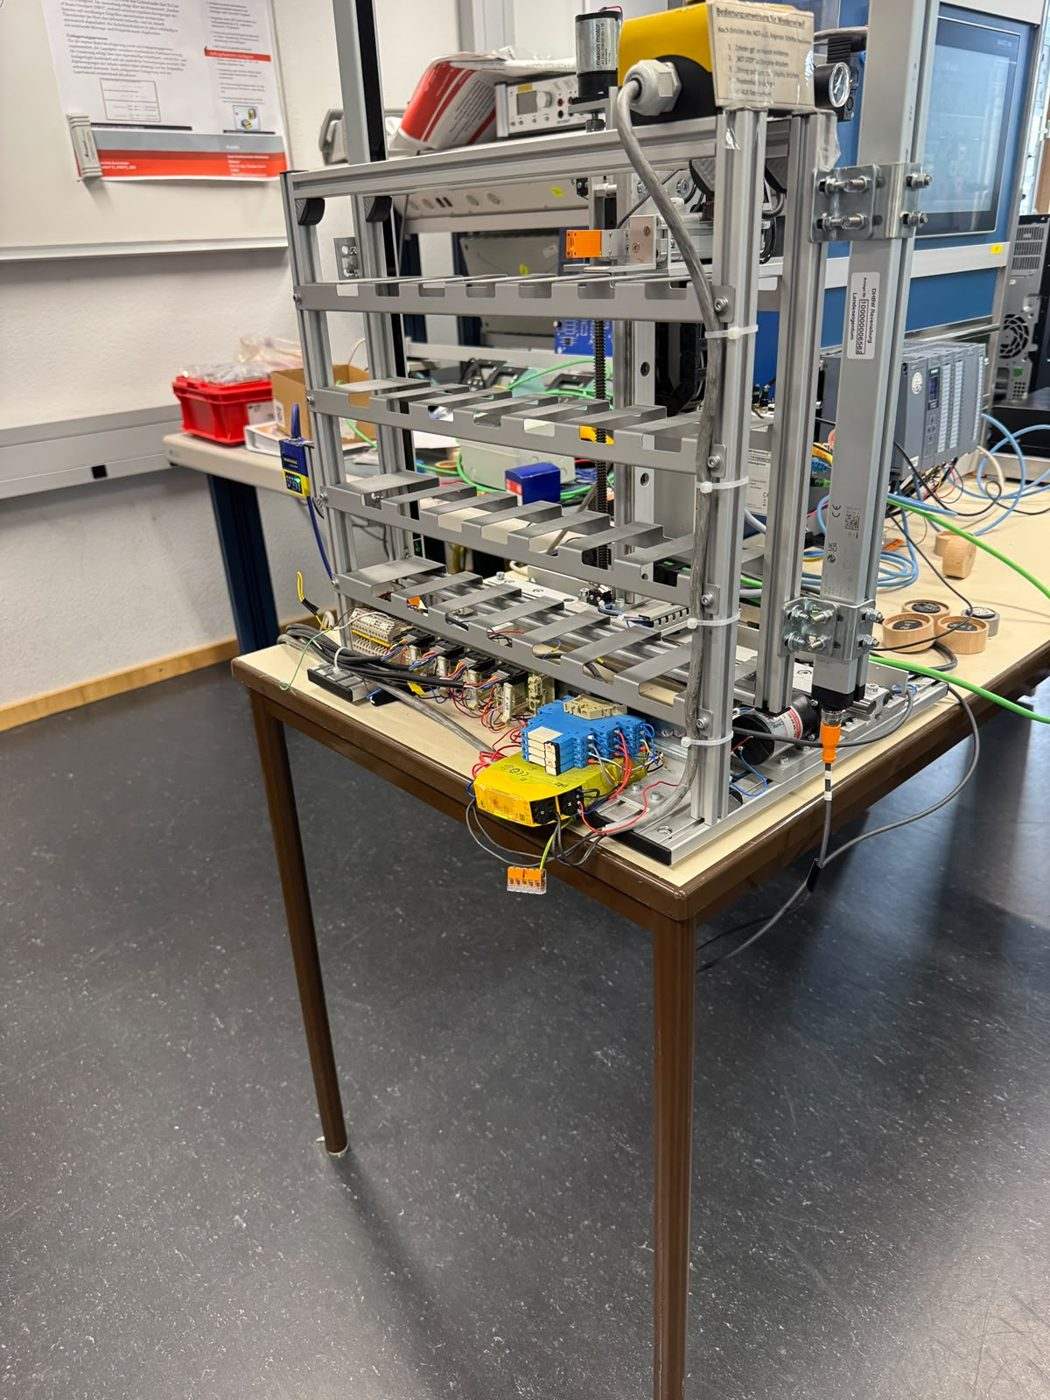
\includegraphics[height=0.4\textheight, trim=6cm 1cm 3cm 0cm, clip]{images/pnoz_ist_position_regal.jpg}
  \caption{Provisorische Position des PNOZ s4 am Prototyp (Ist-Zustand) \quelle{(eigene Aufnahme, 11/2026)}}
  \label{fig:pnoz_ist_position}
\end{figure}

\begin{figure}[H]
  \centering
  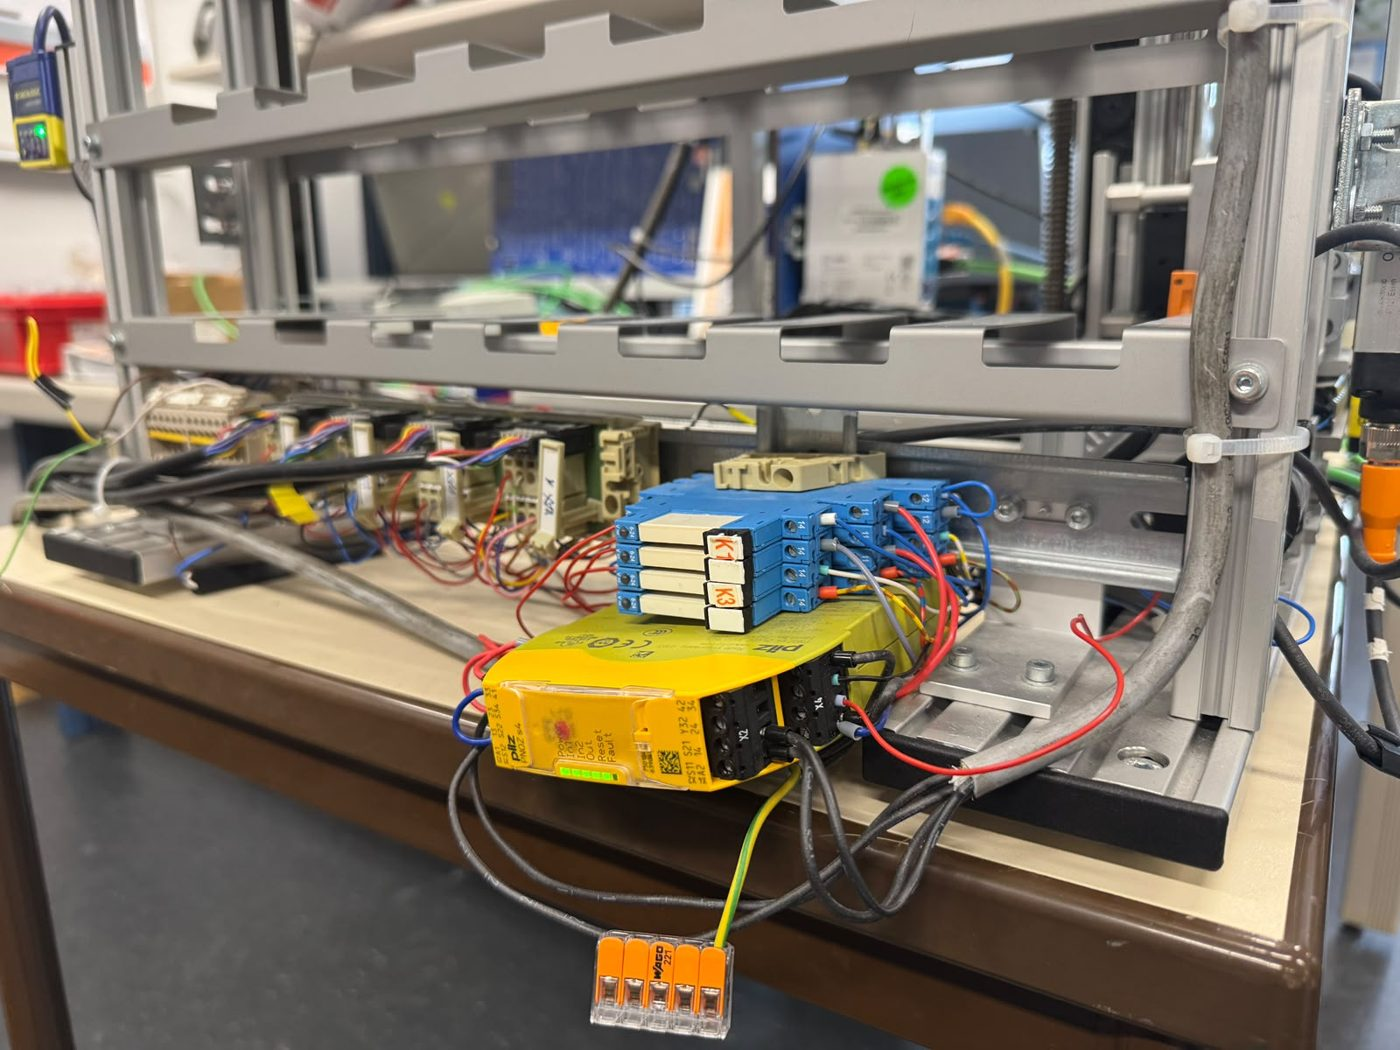
\includegraphics[width=\imgbig]{images/pnoz_ist_montage.jpg}
  \caption{PNOZ s4 neben den Koppelrelais K1--K4,  \quelle{(eigene Aufnahme, 11/2026)}}
  \label{fig:pnoz_ist_montage}
\end{figure}

\begin{figure}[H]
  \centering
  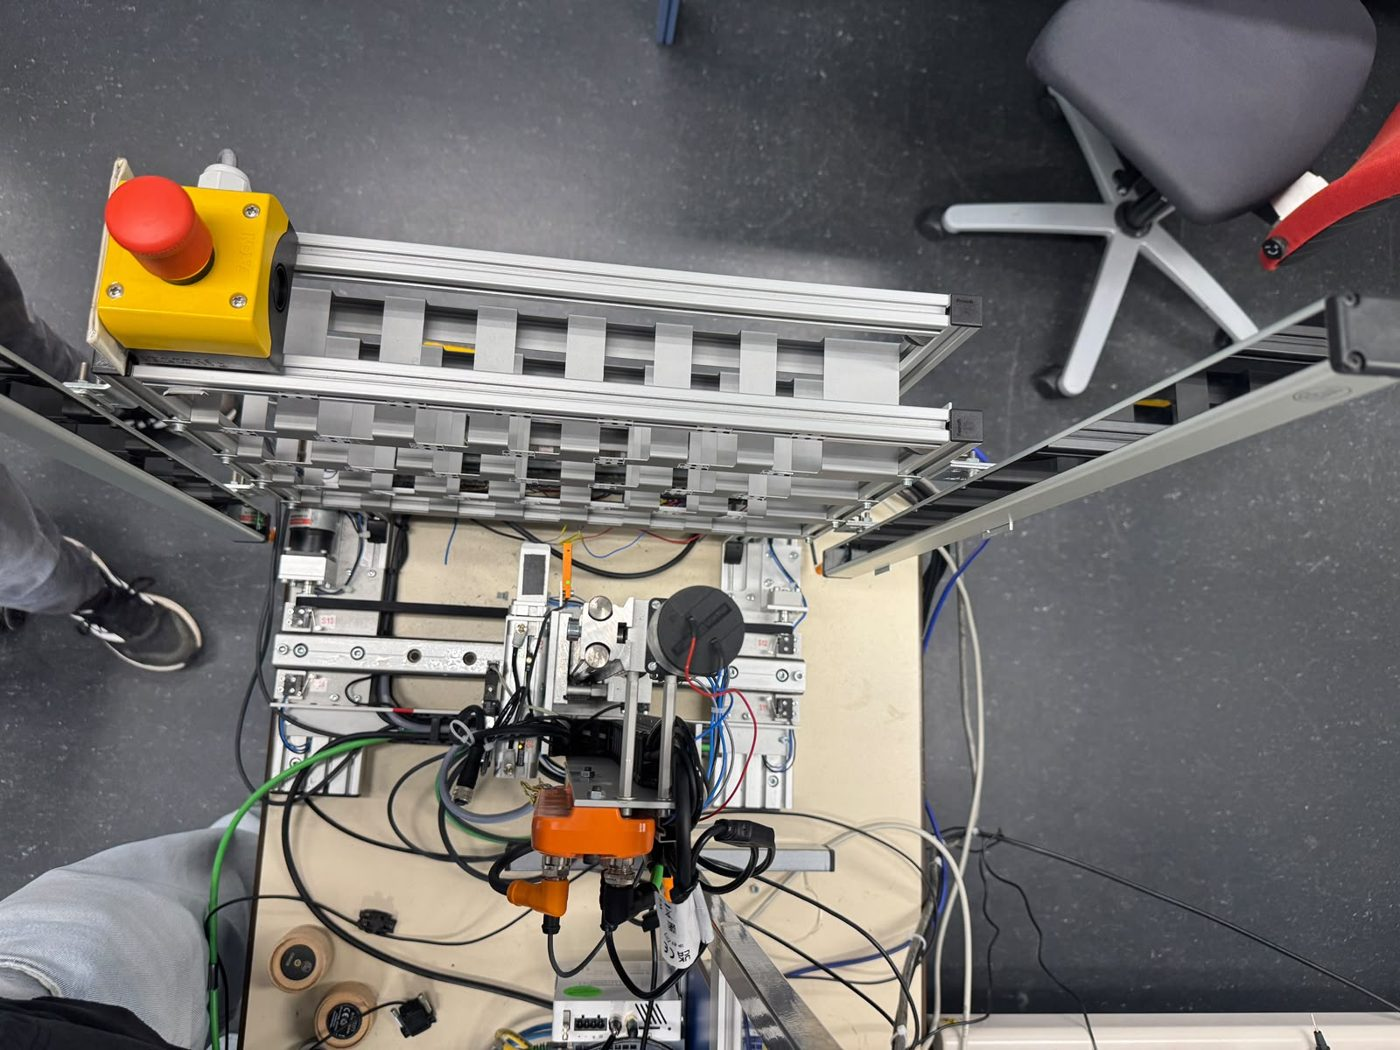
\includegraphics[width=\imgbig]{images/not_halt_taster.jpg}
  \caption{Not-Halt-Taster am Hochregallager (Draufsicht) \quelle{(eigene Aufnahme, 11/2026)}}
  \label{fig:not_halt}
\end{figure}

% TODO: Foto prüfen: Zeigt es das Ventil auf dem Bauteilträger? Nein es zeigt die schlechte Kabelführung an der Schleppkette mit sehr vielen kabeln.
\begin{figure}[H]
  \centering
  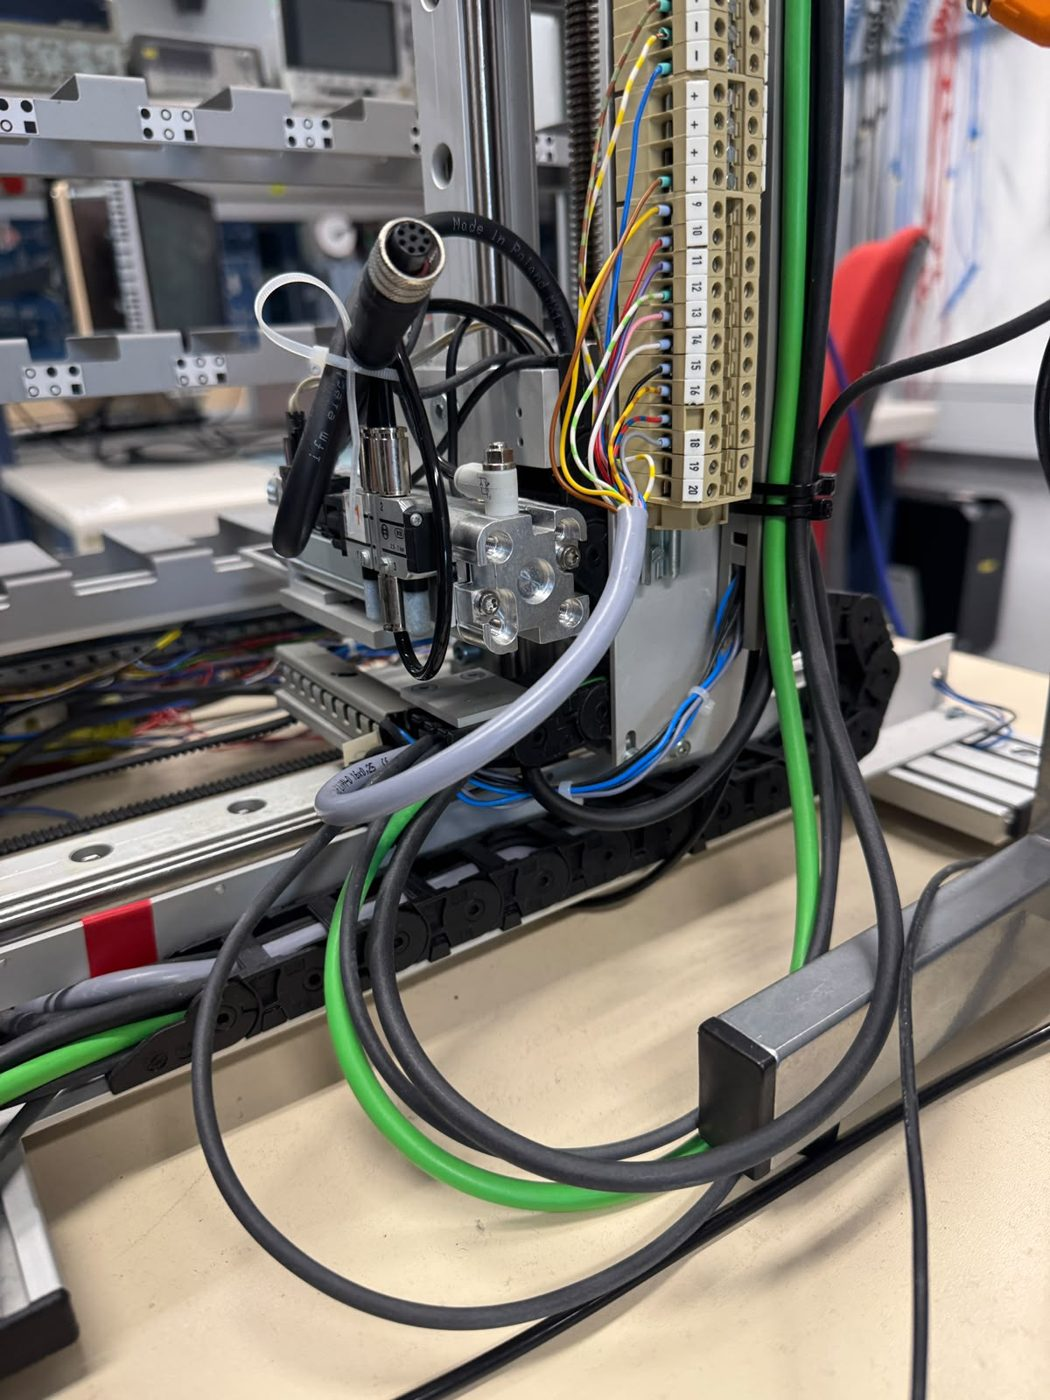
\includegraphics[height=0.4\textheight]{images/druckluftventil_zylinder.jpg}
  \caption{Magnetventil (Bosch, 24\,V DC) \quelle{(eigene Aufnahme, 11/2026)}}
  \label{fig:ventil}
\end{figure}

\subsection{Anforderungen an den neuen Montageort}
% ZIEL:    Kriterien, nach denen der neue Ort gewählt wurde.
% INHALT:  - Steuerungsgestell neben dem Prototyp (dort auch SPS, Switch, Konverter)
%          - Normhutschiene TS35 mit ausreichend Platz, Einbaulage/Abstände laut Handbuch
%          - Zugänglichkeit, saubere Leitungsführung, Zugentlastung, Kennzeichnung
%          - Leitungslängen zu Not-Halt und Motoren
% UMFANG:  ca. 0,5–1 Seite

Als neuer Montageort wird die Hutschiene auf dem Bauteilträger rechts neben dem Switch gewählt. Die Betriebsanleitung fordert eine Montage auf einer 35-mm-Hutschiene \cite{pilz_pnoz_s4}. Der Platz muss eine übersichtliche Leitungsführung und einen guten Zugang zu den Klemmen ermöglichen.

Die Betriebsanleitung sieht außerdem den Einbau in einen Schaltschrank mit mindestens Schutzart IP54 vor \cite{pilz_pnoz_s4}. Der offene Bauteilträger erfüllt diese Vorgabe nicht. Diese Abweichung wird mit dem Betreuer abgestimmt.
% TODO: Ergebnis der Abstimmung ergänzen.

Durch die neue Position werden längere Leitungen zum Not-Halt-Taster und zu den Motoren benötigt. Dafür sind zwei fünfadrige Leitungen mit je 3\,m Länge vorgesehen. Vier Adern verbinden die jeweiligen Schalter des Not-Halts. Vier weitere Adern eines Kabels verbinden die Kontakte 13/14 und 23/24 zu den motoren und den Koppelrelais.
% TODO: Leitungstyp und Querschnitt ergänzen (zulässig laut Anleitung: 0,25--2,5 mm², Kupfer, 75 °C).

\subsection{Prüfung der bestehenden Verdrahtung}
% ZIEL:    Nachweis, dass das Relais korrekt angeschlossen ist – bzw. dokumentierte Abweichungen.
% INHALT:  - Tabelle Ist-Belegung je Klemme vs. Vorgabe/Anschlussbeispiel der Betriebsanleitung
%            (A1, A2, S11/S12, S21/S22, S34, 13/14, 23/24, 33/34, 41/42, Y32)
%          - Bewertung je Klemme: korrekt / Abweichung / offen
%          - Befunde sachlich dokumentieren, z. B. Start-Art (Brücke S12–S34), Absicherung,
%            Kontaktbelastung durch Motoren – mit Empfehlung, aber ohne Umkonzeption
%          - Abstimmung der Befunde mit Prof. Kever
% QUELLEN: Betriebsanleitung PNOZ s4 (Anschlussbeispiele, technische Daten)
% UMFANG:  ca. 1,5 Seiten
% HINWEIS: Klemmenfunktionen nur aus dem Handbuch belegen, nicht aus dem Gedächtnis.

Die Verdrahtung wird Klemme für Klemme mit der Betriebsanleitung \cite{pilz_pnoz_s4} verglichen. Tabelle~\ref{tab:pnoz_klemmen} zeigt das Ergebnis.

\begin{table}[H]
  \centering
  \caption{Vergleich der Ist-Belegung des PNOZ s4 mit der Betriebsanleitung (vorläufig, am Gerät zu bestätigen)}
  \label{tab:pnoz_klemmen}
  \begin{tabular}{|p{1.7cm}|p{4.2cm}|p{4.2cm}|p{3.5cm}|}
    \hline
    \textbf{Klemme} & \textbf{Ist-Belegung} & \textbf{Funktion laut Anleitung} & \textbf{Bewertung} \\ \hline
    A1, A2 & 24\,V, 0\,V & Versorgung & korrekt \\ \hline
    S11/S12, S21/S22 & Not-Halt, zweikanalig & Eingangskreis Kanal 1 und 2 & korrekt \\ \hline
    S34 & mit S12 gebrückt & Start-/Rückführkreis & Befund: Startart \\ \hline
    13/14 & Motor horizontale Achse & Sicherheitskontakt & Befund: Belastung, Redundanz \\ \hline
    23/24 & Motor vertikale Achse & Sicherheitskontakt & Befund: Belastung, Redundanz \\ \hline
    33/34 & 24\,V, Druckluftventil & Sicherheitskontakt & korrekt \\ \hline
    41/42 & 41 an 24\,V, 42 offen & Hilfskontakt, nur für Meldungen & ohne Funktion \\ \hline
    Y32 & nicht belegt & Halbleiterausgang, nur für Meldungen & ohne Funktion \\ \hline
  \end{tabular}
\end{table}

Aus dem Vergleich ergeben sich vier Befunde:

\textbf{Startart:} Durch die Brücke zwischen S12 und S34 ist vermutlich ein automatischer Start eingestellt. Nach dem Entriegeln des Not-Halts schließen die Sicherheitskontakte dann ohne separate Quittierung. Die Betriebsanleitung weist darauf hin, dass in diesem Fall Maßnahmen gegen einen unerwarteten Wiederanlauf vorzusehen sind \cite{pilz_pnoz_s4}.
% TODO: Stellung des Drehschalters „mode“ am Gerät ablesen und ergänzen.

\textbf{Redundanz:} Jeder Motor wird nur über einen Sicherheitskontakt getrennt. Der Eingangskreis ist zweikanalig ausgeführt, die Abschaltung der einzelnen Motoren dagegen einkanalig.

\textbf{Kontaktbelastung und Absicherung:} Die Sicherheitskontakte sind bei 24\,V DC für induktive Lasten (DC-13) mit bis zu 5\,A ausgelegt, abhängig von der Gerätevariante \cite{pilz_pnoz_s4}. Bei induktiven Lasten fordert die Anleitung eine geeignete Schutzbeschaltung. Eine Schutzbeschaltung und eine Kontaktabsicherung sind bisher nicht dokumentiert.
% TODO: Motorstrom messen und mit dem Grenzwert vergleichen; Absicherung am Gerät prüfen.

\textbf{Versorgung:} Das Netzteil liefert laut Datenblatt 3\,A. Ob dieser Strom für alle Verbraucher einschließlich der Motoren ausreicht, wird durch eine Strommessung im Fahrbetrieb geprüft.
% TODO: Messergebnis ergänzen.

Die Befunde werden mit dem Betreuer besprochen. Die Verdrahtung bleibt zunächst unverändert.

\subsection{Montage am neuen Ort}
% INHALT:  - Vorgehen Schritt für Schritt inkl. Sicherheitsmaßnahmen
%          - Aufbau auf der Hutschiene (Foto/Skizze), Leitungsführung, Klemmen/Kennzeichnung
%          - Fotos vorher/nachher als Gegenüberstellung
% UMFANG:  ca. 1 Seite

Vor dem Umbau wird die Anlage freigeschaltet, gegen Wiedereinschalten gesichert und die Spannungsfreiheit festgestellt. Der Ist-Zustand wird mit Fotos und Klemmenbelegung dokumentiert, die Leitungen werden gekennzeichnet.

Anschließend wird das Relais vom Prototyp gelöst und auf der Hutschiene rechts neben dem Switch montiert. Die neuen Leitungen werden zum Not-Halt-Taster und zu den Motorkreisen verlegt und entsprechend der dokumentierten Belegung angeschlossen. Die Leitungen werden zugentlastet und beschriftet.
% TODO: Foto nach dem Umbau ergänzen (Gegenüberstellung vorher/nachher).

\subsection{Funktionsprüfung}
% INHALT:  - einfacher Funktionstest nach dem Umsetzen: funktioniert die Anlage wie vorher?
%            (Not-Halt drücken → Motoren stoppen; entriegeln → Anlage wieder betriebsbereit)
%          - kurz festhalten: Datum, wer, Ergebnis (kleine Tabelle mit 2–3 Zeilen reicht)
% UMFANG:  ca. 0,25 Seiten

Nach dem Umbau wird die Sicherheitsfunktion geprüft. Tabelle~\ref{tab:pnoz_test} enthält die vorgesehenen Prüfschritte.

\begin{table}[H]
  \centering
  \caption{Funktionsprüfung des Sicherheitsrelais (09.11.2026)}
  \label{tab:pnoz_test}
  \begin{tabular}{|p{5.2cm}|p{6.2cm}|l|}
    \hline
    \textbf{Prüfschritt} & \textbf{Erwartung} & \textbf{Ergebnis} \\ \hline
    Not-Halt bei fahrender horizontaler Achse & Motor stoppt, keine Bewegung trotz Fahrbefehl & Erwartung erfüllt
    Not-Halt bei fahrender vertikaler Achse & Motor stoppt, keine Bewegung trotz Fahrbefehl & Erwartung erfüllt
    Pneumatik bei betätigtem Not-Halt & Druckluftkreis ist drucklos & Erwartung erfüllt\\ \hline
    Not-Halt entriegeln & Verhalten wird dokumentiert, keine unerwartete Bewegung & Erwartung erfüllt \\ \hline
    Normalbetrieb nach dem Umbau & Ein- und Auslagern wie vor dem Umbau & Erwartung erfüllt \\ \hline
  \end{tabular}
\end{table}

\subsection{Fazit}
% INHALT:  Relais umgesetzt und geprüft? Offene Befunde/Empfehlungen, Überleitung zu Kapitel 5

Das Sicherheitsrelais wurde an einen geeigneten Montageplatz auf dem Bauteilträger montiert und auf korrekte Verdrahtung geprüft. Die Prüfung verlief erwartungsgemäß. Eine Rückmeldung des Relaiszustands an die SPS ist nicht Teil dieser Arbeit und wird im Ausblick aufgegriffen. Das folgende Kapitel beschreibt die Umstellung des QR-Code-Scanners auf Ethernet.
